\begin{figure}[htb]
\vspace{-0.1cm}
    \begin{center}
    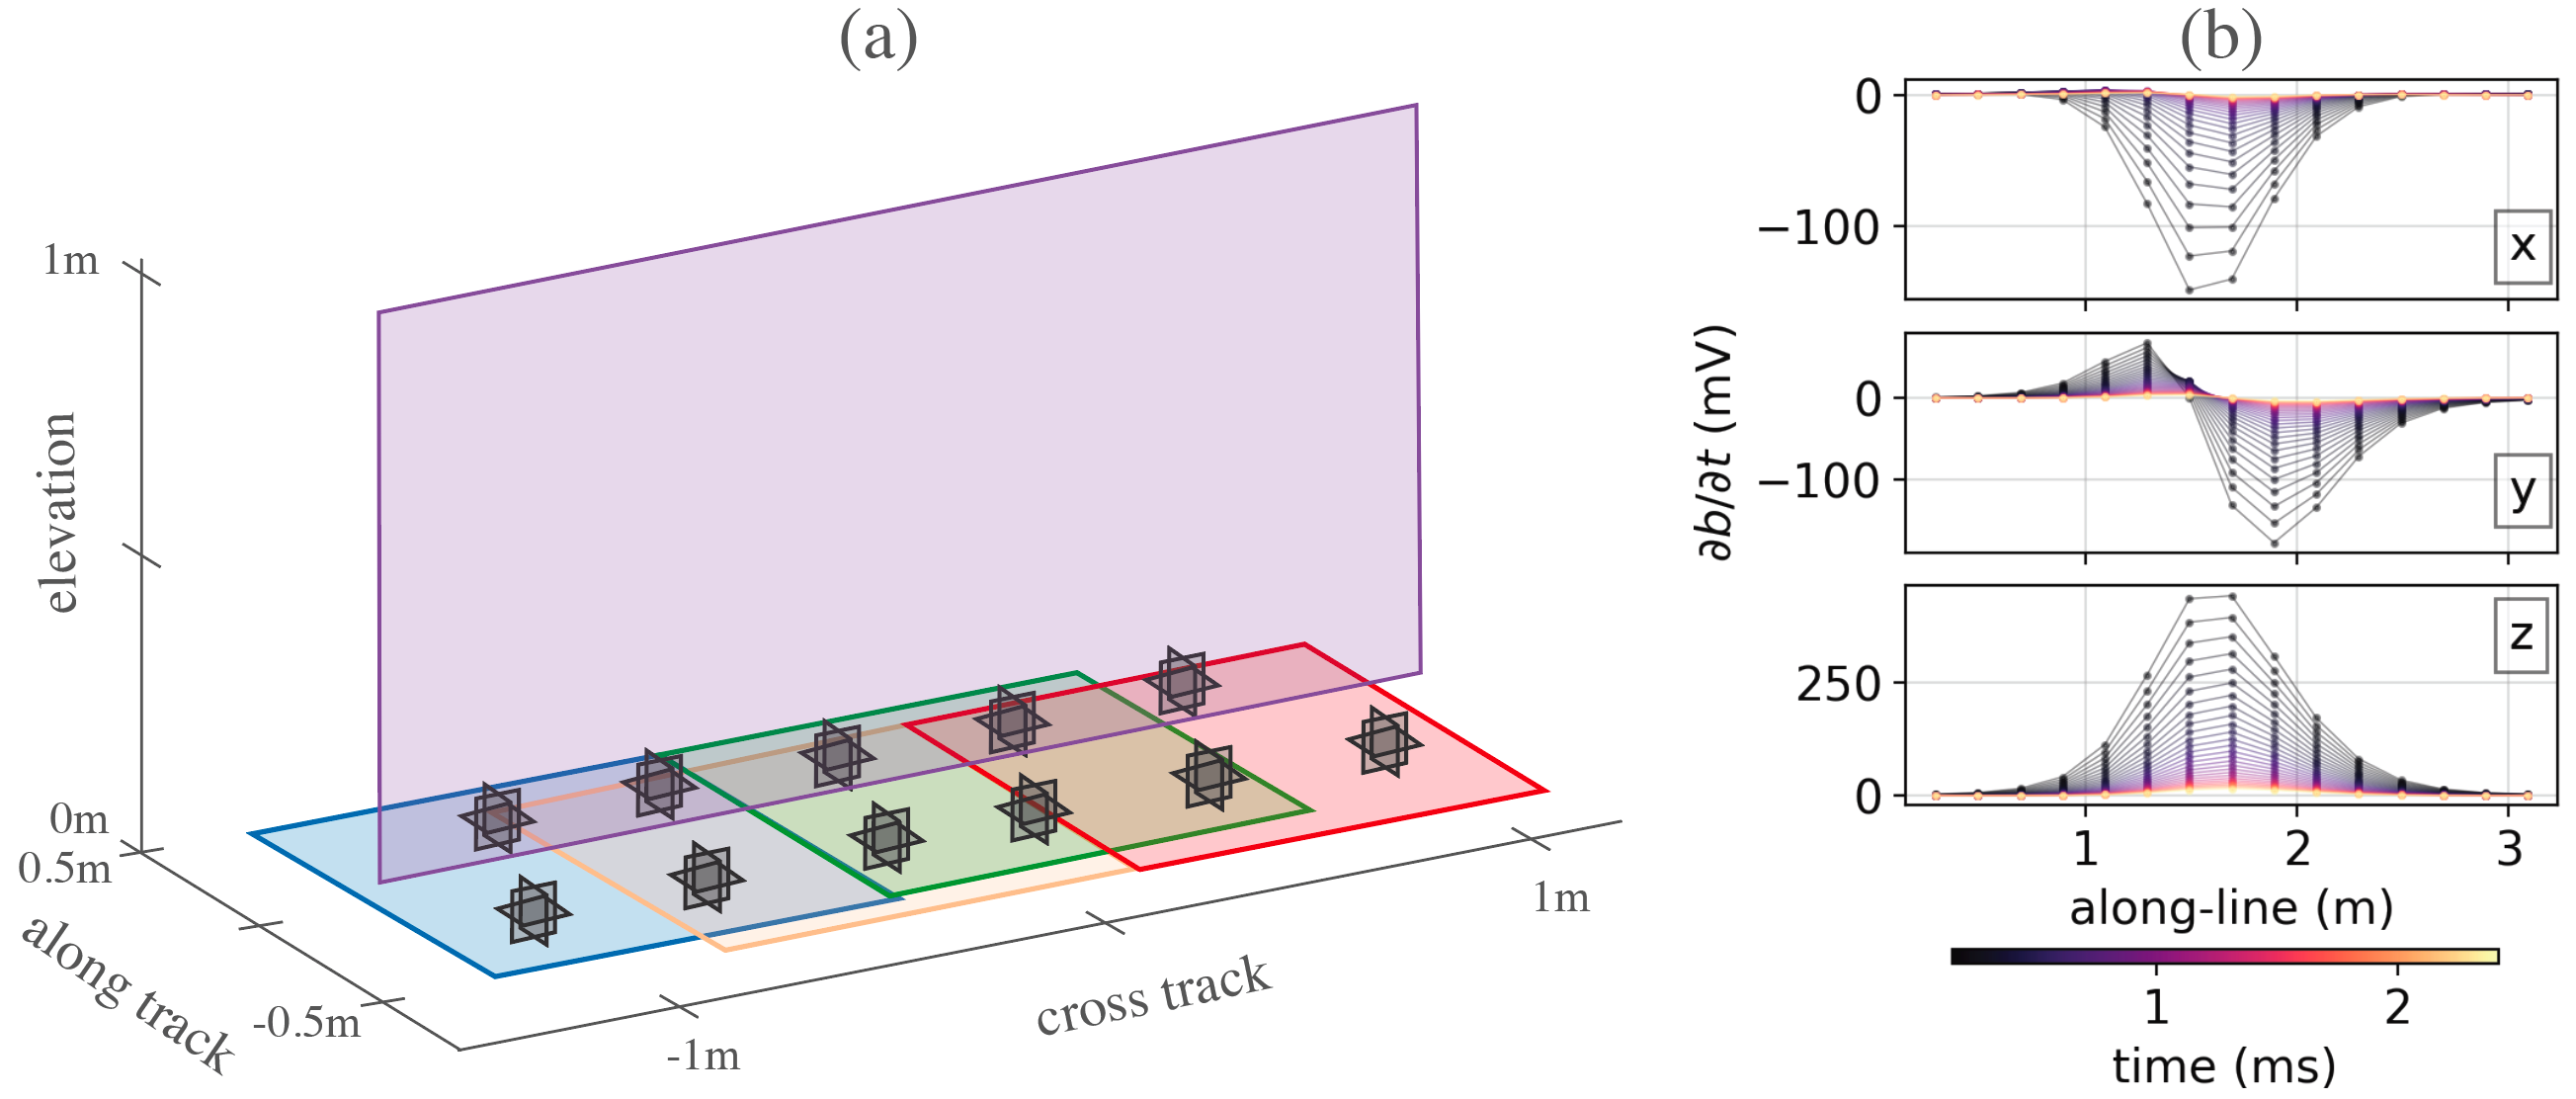
\includegraphics[width=\columnwidth]{figures/ultratem-04.png}
    \end{center}
    \vspace{-0.5cm}
\caption{
    (a) Geometry of the UltraTEM system. Colors indicate transmitters
    and the grey cubes are the three-component $\partial \mathbf{b}/\partial t$ receivers.
    (b) A sample of simulated data (one transmitter and one 3-component receiver) over a Medium ISO. The color of the lines indicates the time-channel.
}
\label{fig:ultratem}
\vspace{-0.1cm}
\end{figure}
